%卒論概要テンプレート ver. 4.0

\documentclass[uplatex,twocolumn,dvipdfmx]{jsarticle}
\usepackage[top=22mm,bottom=22mm,left=22mm,right=22mm]{geometry}
\setlength{\columnsep}{11mm}
\usepackage[T1]{fontenc}
\usepackage{txfonts}
\usepackage[expert,deluxe]{otf}
\usepackage[dvipdfmx,hiresbb]{graphicx}
\usepackage[dvipdfmx]{hyperref}
\usepackage{pxjahyper}
\usepackage{secdot}





%タイトルと学生番号,名前だけ編集すること
\title{\vspace{-5mm}\fontsize{14pt}{0pt}\selectfont 分散型SNSにおけるユーザの潜在要求分析}
\author{\normalsize プロジェクトマネジメントコース 矢吹研究室 1442037 加藤 健弥}
\date{}
\pagestyle{empty}
\begin{document}
\fontsize{10.5pt}{\baselineskip}\selectfont
\maketitle





%以下が本文
\section{序論}\label{序論}
スマートフォンなどの普及により,手軽にインターネットへの接続が可能になった.そのため,TwitterやFacebookなどの様々なSNS(ソーシャルネットワークサービス)が注目されるようになった.近年ではMastodonという新たなSNSの利用者が増えてきている.

Mastodonとは2016年に公開されたフリーソフトウェアであり,サーバを立てることが出来れば誰でもMastodonを自由に運用することが可能である.そのため,TwitterやFacebookのような利用者が一つのサーバにログインする中央集権型のサービスに対してMastodonでは管理者も設置場所も異なるサーバで運用できる.したがって利用者は自分自身でサーバを選びアカウントを作成してログインする.Mastodonではこのサーバのことを「インスタンス」と呼び,その中で利用者がつぶやきを投稿することを「トゥート」と呼ぶ\cite{wiki}.


\section{目的}

Mastodonのインスタンスごとのつぶやきを定量的に分析し,その結果からインスタンスごとに話題が異なっているかを調査する.

\section{手法}

Mastodon APIを使用し,複数のMastodonのインスタンスからつぶやきを集めてベクトル化する.その結果を主成分分析する.


\section{結果}

Mastodonの一つのインスタンスから無作為に100のつぶやきを抽出し,つぶやきのベクトル化を行った.計30のインスタンスでつぶやきのベクトル化を行い,その結果を主成分分析した.図\ref{mstdn}は話題が自由なインスタンスであるmstdn.jpのつぶやきをベクトル化し,主成分分析をした結果である.図\ref{ika}はスプラトゥーンの話題が中心のインスタンスであるika.queloud.netのつぶやきをベクトル化し,主成分分析した結果である.
\begin{figure}[h]
\begin{tabular}{cc}
\begin{minipage}{0.5\hsize}
\begin{center}
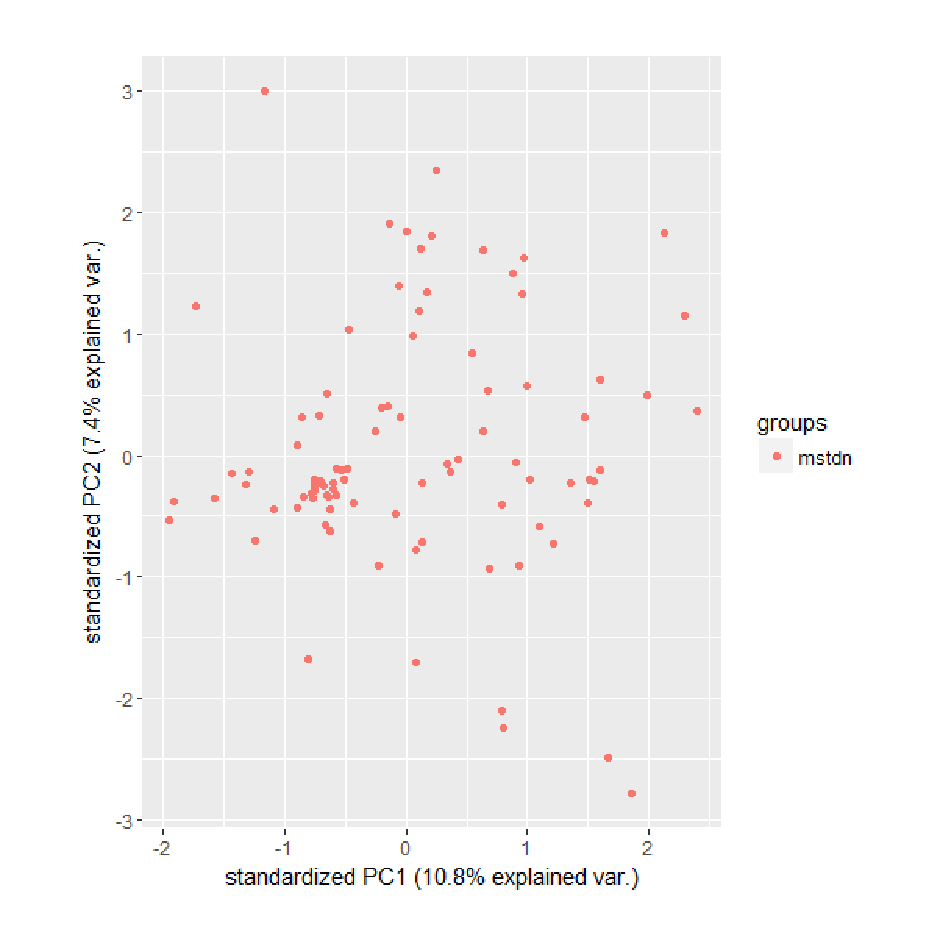
\includegraphics[width=50mm,clip]{mstdn.pdf}
\caption{話題が自由なインスタンス}
\label{mstdn}
\end{center}
\end{minipage}
\begin{minipage}{0.5\hsize}
\begin{center}
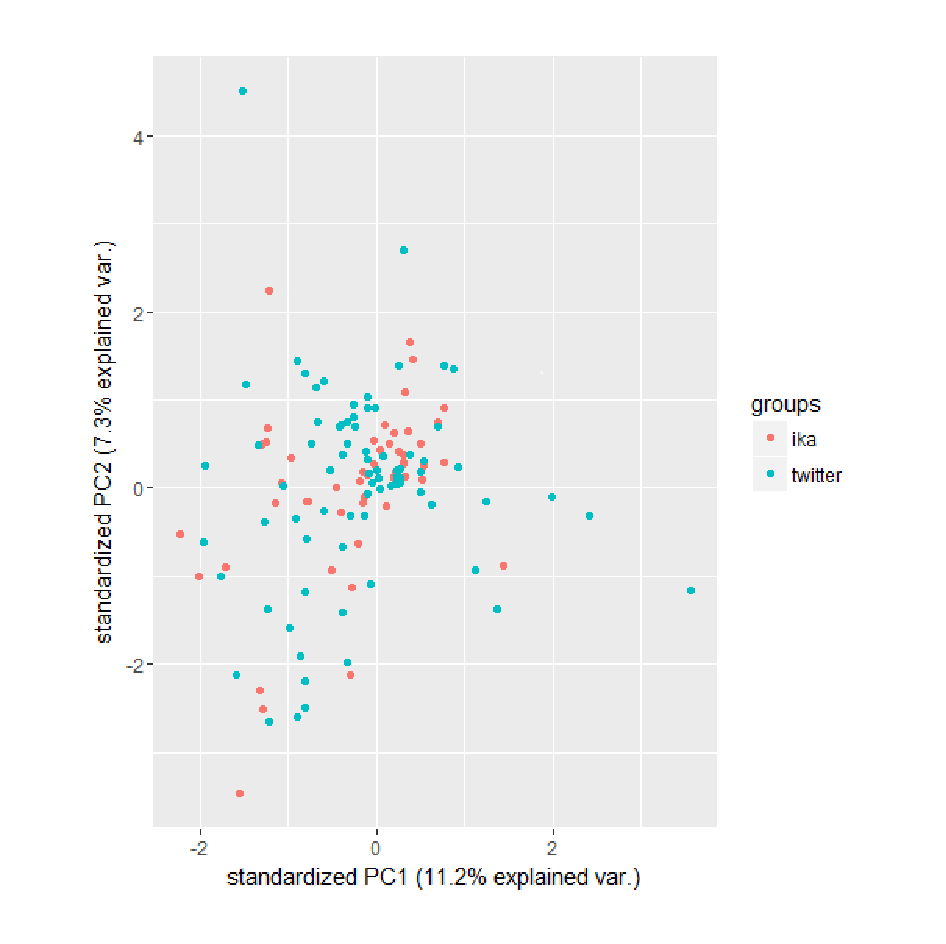
\includegraphics[width=50mm,clip]{ika.pdf}
\caption{スプラトゥーンが話題の中心のインスタンス}
\label{ika}
\end{center} 
\end{minipage}
\end{tabular}
\end{figure}
\section{考察}

インスタンスごとにつぶやきを定量化した結果,話題が細かく設定されているインスタンスほどばらつきが少ないと感じた.そういったインスタンスは人間の目から見ても共通の話題でつぶやかれていると考えられる.話題が広く設定されているインスタンスではばらつきがあると感じた.そういったインスタンスは人間の目から見ても異なった話題でつぶやかれていると考えられる.しかし人間の目から見ても話題が共通しているインスタンスにもばらつきがみられたため,機械による判別が精度が低いと考えられる.

\section{結論}

Mastodonの異なるインスタンスごとに共通の話題のつぶやきがされているか定量的に分析した.人間の目でみて共通の話題をしているインスタンスであっても定量的に分析し,判別することへの精度が低いとわかった.今後は略称や愛称などの自然言語処理の精度を高めることで精度の高い判別を行えると考えられる.

\bibliographystyle{junsrt}
\bibliography{biblio}%「biblio.bib」というファイルが必要.

\end{document}